\documentclass[10pt]{article}
\usepackage[margin=1in]{geometry}
\usepackage{amsmath,amssymb,amsfonts,amsthm}
\usepackage{graphicx}
\usepackage{booktabs}
\usepackage{algorithm}
\usepackage{algpseudocode}
\usepackage[colorlinks=true,linkcolor=blue,citecolor=blue]{hyperref}
\usepackage{caption}
\captionsetup{font=small,labelfont=bf}

\theoremstyle{definition}
\newtheorem{definition}{Definition}
\theoremstyle{plain}
\newtheorem*{thmA}{Theorem 3.1 (Li et al., informal)}
\newtheorem*{thmB}{Theorem 4.1 (Li et al.)}
\newtheorem*{thmC}{Theorem 5.1 (Li et al.)}
\newtheorem*{thmD}{Theorem 5.2 (Li et al.)}
\newtheorem*{thmE}{Theorem 6.1 (Li et al.)}
\newtheorem*{asmA}{Assumption 2.1 (Li et al.)}
\newtheorem*{asmB}{Assumption 2.2 (Li et al.)}

\newcommand{\shat}{\hat{s}}
\newcommand{\pdata}{p_{\mathrm{data}}}
\newcommand{\mdata}{\mu_{\mathrm{data}}}
\newcommand{\R}{\mathbb{R}}
\newcommand{\E}{\mathbb{E}}
\newcommand{\TM}{\mathcal{T}_M}
\newcommand{\dM}{d_M}

\title{Tempered Guided Sampling of the Uniform Measure\\on a Conditional Submanifold: Experiments on $S^3$}
\author{}
\date{}

\begin{document}
\maketitle
\vspace{-3em}

\begin{abstract}
\noindent
We test whether the rate separation of \emph{When Scores Learn Geometry}
(Li, Shen, Hsieh \& He, arXiv:2509.24912) extends from a data manifold $M$ to a
\emph{conditional submanifold} $N = M \cap H$ cut out by a hyperplane supplied
at inference. On $S^3 \subset \R^4$ we measure the guidance term to sit at the
\emph{geometric} rate, and show that tempered guided Langevin recovers the
uniform measure on $N$ exactly when the score is exact. With a learned score the
sampler falls short of statistical uniformity at every tempering exponent, for a
reason the theory does not model: the exponent required by the error condition
and the exponent at which the sampler leaves the training distribution overlap
only marginally.
\end{abstract}

\section{Definitions}

We follow the notation of Li et al.\ throughout.

\begin{definition}[Manifold, chart, volume measure]
$M \subset \R^d$ is a compact boundaryless $C^4$ embedded submanifold of
dimension $n$ and codimension $c = d-n$. A chart is a smooth map
$\Phi : U \to M$, $U \subset \R^n$, with Riemannian metric tensor $g(u)$. The
Riemannian volume measure satisfies
$\int_M f\, \mathrm{d}M = \int_U f(\Phi(u)) \sqrt{\det g(u)}\, \mathrm{d}u$;
the \emph{uniform measure on $M$} is the normalised $\mathrm{d}M$, i.e.\ density
$\propto \sqrt{\det g(u)}$ in local coordinates.
\end{definition}

\begin{definition}[Tubular neighbourhood, projection, squared distance]
$\TM(\epsilon) := \{x \in \R^d : \mathrm{dist}(x,M) < \epsilon\}$. For
$\epsilon$ below the reach, each $x \in \TM(\epsilon)$ has a unique nearest
point $P_M(x) \in M$, and
$\dM(x) := \tfrac12 \mathrm{dist}^2(x,M) = \min_{\bar{x}\in M} \tfrac12\|x-\bar x\|^2$.
\end{definition}

\begin{definition}[Smoothed measure; VE process]
For $\mdata$ on $M$ with density $\pdata$ w.r.t.\ $\mathrm{d}u$, the
variance-exploding smoothing is $X_\sigma = X_0 + \sigma Z$,
$X_0 \sim \mdata$, $Z \sim \mathcal{N}(0,I_d)$, with density
\begin{equation}
p_\sigma(x) \;=\; \int_M \frac{1}{(2\pi\sigma^2)^{d/2}}
  \exp\!\Big(-\tfrac{\|x - \Phi(u)\|^2}{2\sigma^2}\Big)\, \pdata(u)\, \mathrm{d}u .
\end{equation}
\end{definition}

\begin{definition}[Score, hat score, score error]
The ideal score is $s^*(x,\sigma) := \nabla \log p_\sigma(x)$; a learned oracle
is $s(x,\sigma)$. The \emph{hat score} (Tweedie displacement) is
\begin{equation}
\shat(x,\sigma) \;:=\; \sigma^2\, \nabla \log p_\sigma(x)
   \;=\; \E[X_0 \mid X_\sigma = x] - x ,
\label{eq:hat}
\end{equation}
which is $O(\sigma)$ on $\TM(\epsilon)$ and hence numerically stable at small
$\sigma$. The score error is
$E_\sigma := \|s(\cdot,\sigma) - s^*(\cdot,\sigma)\|_{L^\infty(K)}$ for a compact
$K \supset \TM(\epsilon)$. A hat error $\hat{e}$ corresponds to raw error
$\hat{e}/\sigma^2$.
\end{definition}

\begin{definition}[Tempered Score Langevin, eq.~(8) of Li et al.]
For $\alpha > 0$,
\begin{equation}
\mathrm{d}X_t \;=\; \sigma^{\alpha}\, s(X_t,\sigma)\, \mathrm{d}t
   \;+\; \sqrt{2}\, \mathrm{d}W_t
   \;=\; \sigma^{\alpha-2}\, \shat(X_t,\sigma)\, \mathrm{d}t + \sqrt2\, \mathrm{d}W_t ,
\label{eq:ts}
\end{equation}
with stationary law $\tilde\pi_\sigma$. Setting $\alpha=0$ recovers the standard
Langevin ``corrector''. Discretised with $\Delta t = \eta\,\sigma^{2-\alpha}$,
the transverse equilibrium width is $\sigma^{1-\alpha/2}$.
\end{definition}

\begin{definition}[Conditional submanifold]
For a unit $w \in \R^d$ drawn at inference, $H := \{x : \langle w,x\rangle = 0\}$
and $N := M \cap H$, of dimension $n-1$ for generic $w$. Conditioning is on the
event $c := \{\langle X_0, w\rangle = 0\}$, of measure zero in $M$; ``uniform on
$N$'' means normalised $\mathrm{d}N$.
\end{definition}

\begin{definition}[Exact guidance for a linear constraint]
Since $x \mapsto \langle w,x\rangle$ is linear, Tweedie \eqref{eq:hat} gives the
posterior mean in closed form,
\begin{equation}
m(x) \;:=\; \E\!\left[\langle w, X_0\rangle \mid X_\sigma = x\right]
   \;=\; \big\langle w,\; x + \shat(x,\sigma) \big\rangle .
\label{eq:mean}
\end{equation}
With $v(x) := \mathrm{Var}[\langle w,X_0\rangle \mid X_\sigma=x] \approx \sigma^2$
and $\nabla m \approx w$, the Gaussian-posterior guidance is
$\nabla \log p_\sigma(c\mid x) \approx -(m/v)\nabla m$, i.e.\ in hat space
$\hat{g} = -m(x)\,w$ and $\shat_c = \shat + \hat{g}$. No classifier is trained.
\end{definition}

\begin{definition}[Uniformity statistics]
For samples $u_i$ on a great $S^2 \subset w^\perp$ with real orthonormal
spherical harmonics $Y_{\ell m}$:
\emph{(i)} the \emph{marginal} deviation is
$\max_k \max_{\text{bin}} |\hat p_k/p_k - 1|$, where $\langle e_k, x\rangle$ is
exactly $\mathrm{Unif}[-1,1]$ under uniformity (Archimedes);
\emph{(ii)} the \emph{harmonic statistic}
$T := 4\pi N_s \sum_{\ell=1}^{L}\sum_{m} \bar{Y}_{\ell m}^2$, which is
$\chi^2_{L(L+2)}$ under uniformity ($L=6$, $\mathrm{dof}=48$), rotation
invariant, with per-$\ell$ power localising the defect;
\emph{(iii)} the \emph{dipole} $|\bar{u}|$, the centroid length, the $\ell=1$
mode, with empirical null $0.0062 \pm 0.0025$ at $N_s = 20000$.
\end{definition}

\begin{definition}[Exploration metrics]
On $K^2$ equal-area cells of $N$: the KL divergence to uniform (bias-corrected),
and the \emph{rare-region mass}, the sample mass falling in the decile of cells
where $\pdata|_N$ is smallest. The latter is the operational objective when the
goal is manifold exploration rather than a hypothesis test.
\end{definition}

\section{Recalled results}

\begin{asmA}[Manifold hypothesis]
$\mdata$ is supported on a compact, boundaryless $C^4$ embedded submanifold
$M \subset \R^d$ with $\dim(M) = n$.
\end{asmA}

\begin{asmB}[Regularity and coverage]
$\pdata : U \to \R$ w.r.t.\ Lebesgue measure on $U$ is $C^1(U)$ and strictly
positive.
\end{asmB}

\begin{thmA}[Scale separation]
Under Assumptions 2.1--2.2, for any $x \in \TM(\epsilon)$,
\begin{equation}
\log p_\sigma(x) \;=\; -\frac{1}{\sigma^2}\dM(x)
  \;+\; \log \pdata\big(\Phi^{-1}(P_M(x))\big)
  \;-\; \frac{d-n}{2}\log(2\pi\sigma^2) \;+\; H(x) \;+\; o(1),
\label{eq:expansion}
\end{equation}
where $H$ carries curvature information and both $H,\epsilon$ are independent of
$\sigma$; the $o(1)$ is uniform on $\TM(\epsilon)$.
\end{thmA}

\noindent
Geometry enters at $\Theta(\sigma^{-2})$ and the density only at $\Theta(1)$:
the separation this paper is built on.

\begin{thmB}[Rate separation in recovery]
Under Assumptions 2.1, 2.2, 4.1, with $E_\sigma$ the score error:
\emph{(1) Concentration.} If $E_\sigma = o(\sigma^{-2})$ then $\pi_\sigma$
concentrates on $M$.
\emph{(2) Arbitrary recovery.} For any $\hat\pi$ on $M$ with $C^1$ density one
can construct $f_\sigma$ with $E_\sigma = \Omega(1)$ and
$\pi_\sigma \rightharpoonup \hat\pi$.
\emph{(3) Recovering $\pdata$.} If $E_\sigma = o(1)$ then
$\pi_\sigma \rightharpoonup \pdata$.
\end{thmB}

\begin{thmC}[TS Langevin samples the uniform measure]
Assume Assumptions 2.1, 2.2, 4.1 (with $\pi_\sigma$ replaced by
$\tilde\pi_\sigma$). Suppose
\begin{equation}
\|s(x,\sigma) - s^*(x,\sigma)\|_{L^\infty(K)} = o(\sigma^{\beta})
\quad\text{for some } \beta > -2 .
\label{eq:err}
\end{equation}
Then for any $\max\{-\beta,0\} < \alpha < 2$, as $\sigma \to 0$,
$\tilde\pi_\sigma$ converges weakly to the uniform distribution on $M$ w.r.t.\
the intrinsic volume measure: $\tilde\pi(u) \propto \sqrt{\det g(u)}$.
\end{thmC}

\begin{thmD}[Non-gradient oracle]
Assume Assumptions 2.1--2.2 and \eqref{eq:err}, with $\pdata \in C^2(U)$. For any
$\max\{-\beta,0\} < \alpha < 2$, if the SDE admits a unique stationary
distribution locally of WKB form with $\theta = \sigma^{2-\alpha}$, the
conclusion of Theorem 5.1 holds.
\end{thmD}

\begin{thmE}[Bounded potential / guidance]
Under the assumptions of Theorem 5.2, and $v : \R^d \to \R$ bounded and $C^1$ on
$\TM(\epsilon)$, the stationary distribution of
$\mathrm{d}x_t = -\nabla v\, \mathrm{d}t - \sigma^\alpha \nabla f_\sigma\, \mathrm{d}t + \sqrt2\, \mathrm{d}W_t$
converges weakly to a distribution on $M$ with density
$\propto \exp(-v(\Phi(u)))\, \sqrt{\det g(u)}$.
\end{thmE}

\paragraph{Positioning.} Theorem 6.1 covers a \emph{bounded $C^1$} potential ---
classifier-free guidance reweighting mass \emph{within} $M$ --- and yields
$\exp(-v)\times$volume, not a uniform measure on a smaller set. Our constraint is
a measure-zero event that \emph{adds codimension}; formally it is the limit of
potentials $v_\varepsilon \to \infty$ off $H$, outside the scope of Theorem 6.1.
That regime is what we measure below.

\paragraph{Two exponents.} Condition \eqref{eq:err} couples the admissible
tempering exponent to the score error: a larger error (more negative $\beta$)
\emph{forces a larger} $\alpha$. Section~4 shows that a larger $\alpha$ also
places the sampler's equilibrium cloud further from $M$ in units of $\sigma$,
where a denoising-trained score is less accurate. The theory assumes the bound
in \eqref{eq:err} uniformly on $K$ and so does not see this feedback.

\begin{algorithm}[t]
\caption{Tempered guided Langevin corrector (this work)}
\label{alg:corrector}
\begin{algorithmic}[1]
\Require score oracle $\shat(\cdot,\sigma)$, unit normal $w$, level $\sigma$,
  exponent $\alpha \in (0,2)$, step scale $\eta$, steps $K$,
  init $x_0 \sim \pdata|_N + \sigma\varepsilon$
\State $\Delta t \gets \eta\, \sigma^{2-\alpha}$
\For{$k = 0,\dots,K-1$}
  \State $\shat_k \gets \shat(x_k,\sigma)$
  \State $m \gets \langle w,\, x_k + \shat_k \rangle$
    \Comment{exact posterior mean, Eq.~\eqref{eq:mean}}
  \State $\shat_c \gets \shat_k - m\,w$
    \Comment{guided hat score; $v \approx \sigma^2$, $\nabla m \approx w$}
  \State $x_{k+1} \gets x_k + \sigma^{\alpha-2}\,\shat_c\,\Delta t
     + \sqrt{2\Delta t}\,\xi_k$, \quad $\xi_k \sim \mathcal{N}(0,I)$
\EndFor
\State \Return $x_K$
\end{algorithmic}
\end{algorithm}

\noindent
The drift step is $\eta\,\sigma^{\alpha}\!\cdot\!\Theta(\sigma^{-1})$,
independent of $\sigma$; the equilibrium width is $\sigma^{1-\alpha/2}$ around
both $M$ and $H$. Empirically the stationary law on $N$ is
$\pdata^{\,\sigma^\alpha}$, which sets the finite-$\sigma$ bias --- consistent
with Theorem 5.1, where the bias vanishes only as $\sigma \to 0$. Step counts
are set by simulated time: the $\ell=1$ mode on $N$ decays at rate
$\ell(\ell+1)=2$, so $T$ time units give ${\approx}2.5T$ e-foldings (measured
$2.51$).

\section{Experimental protocol}

$M = S^3 \subset \R^4$; $\pdata$ a three-component von Mises--Fisher mixture
($\kappa \in [1,3]$, density ratio ${\approx}15$). The learned score is a
$384{\times}5$ MLP trained by denoising score matching (60k steps, batch 1024,
$\sigma \in [0.01,10]$ log-uniform, biased toward $\sigma_{\min}$); it passes
seven geometry gates (flow distance $7.9{\times}10^{-4}$, normal angle
$0.93^\circ$, hat error $8.7{\times}10^{-4}$ at $\sigma_{\min}$). The exact
control is the closed-form Bessel score, $z$-tested against Monte Carlo (worst
$|z| = 3.3$ where $\mathrm{ESS}>200$). All runs: $\sigma = 0.01$, $\eta = 0.2$,
$N_s = 20000$, chains initialised at $\pdata|_N$ so the corrector must transport
mass.

\section{Results}

\paragraph{The guidance term sits at the geometric rate.}
Over 50 random hyperplanes with exact scores, fitting
$\log\|\cdot\|$ against $\log\sigma$ on $\sigma \le 0.05$ ($R^2 = 1.0000$): the
geometric term has slope $-0.999 \pm 0.002$, the density term
$-0.001 \pm 0.001$, and the guidance term $\mathbf{-1.000 \pm 0.003}$ for points
near $N$ and $\mathbf{-2.001 \pm 0.003}$ for points on $M$ away from $N$
(Figure~\ref{fig:rates}). Magnitudes are $\Theta(\sigma^{-1})$ where
\eqref{eq:expansion} gives stiffness $\Theta(\sigma^{-2})$, since
$\|\nabla \dM\| = \Theta(\sigma)$ at a typical noised point. Conditioning on a
linear constraint therefore behaves as \emph{geometry}: one exponent suppresses
the density while preserving both $M$ and the constraint.

\begin{table}[h]
\centering\small
\caption{Uniformity on $N$ at $\sigma = 0.01$. $T \sim \chi^2_{48}$ under
uniformity; the exact-uniform control gives $T = 44.1$, $p = 0.63$. ``Bias'' is
the dipole of the empirical stationary law $\pdata^{\,\sigma^\alpha}$.}
\label{tab:main}
\begin{tabular}{llrrrrr}
\toprule
score & $\alpha$ & $T$ & harmonic $p$ & $|$dipole$|$ & bias & verdict \\
\midrule
--- ($\pdata|_N$, start) & --- & 8733.9 & $0$ & 0.354 & --- & --- \\
learned & 0.5 & 487.3 & $5{\times}10^{-74}$ & 0.066 & 0.040 & rejected \\
learned & 0.6 & 523.7 & $3{\times}10^{-81}$ & 0.072 & 0.025 & rejected \\
exact & 0.5 & 142.2 & $3{\times}10^{-11}$ & 0.037 & 0.040 & rejected \\
exact & 0.75 & 59.4 & $0.125$ & 0.010 & 0.012 & \textbf{uniform} \\
exact & 1.0 & \textbf{39.4} & $\mathbf{0.807}$ & 0.007 & 0.003 & \textbf{uniform} \\
exact & 1.25 & 40.8 & $0.760$ & 0.008 & 0.001 & \textbf{uniform} \\
\bottomrule
\end{tabular}
\end{table}

\paragraph{With an exact score, tempering recovers the uniform measure on $N$.}
At $\alpha = 1$ the sample is statistically indistinguishable from uniform
($T = 39.4$ vs.\ the control's $44.1$), removing $99.5\%$ of the harmonic power
of $\pdata|_N$. The residual at $\alpha = 0.5$ is exactly the finite-$\sigma$
bias: dipole $0.037$ against a predicted $0.040$, agreeing in direction to
$\cos\theta = 0.999$. This is Theorem 5.1's conclusion realised at finite
$\sigma$, with $N$ in place of $M$.

\paragraph{The learned score is the binding constraint, via training coverage.}
The equilibrium cloud sits at $\sigma^{-\alpha/2}$ noise lengths from $M$,
independent of $\sigma$. Denoising training places points at
${\approx}\sigma\sqrt{d}$ ($\chi_d$-concentrated), so of $6.1{\times}10^7$
training pairs, ${\sim}2.5{\times}10^6$ reach the $\alpha{=}0.5$ cloud
($3.2\sigma$), ${\sim}140$ reach $\alpha{=}0.75$ ($5.6\sigma$), and effectively
none reach $\alpha{=}1$ ($10\sigma$, $P \approx 10^{-20}$). The learned model's
dipole \emph{excess} over the theoretical bias accordingly grows
($0.052 \to 0.068 \to 0.335$ at $\alpha = 0.5, 0.6, 1$) while the bias shrinks,
so no $\alpha$ attains uniformity; the optimum is near $\alpha \approx 0.5$ at
${\approx}10\times$ the null.

This is the feedback \eqref{eq:err} does not model. Our model's raw error is
$7.2$ at $1\sigma$ and $49$ at $10\sigma$ ($\sigma = 0.01$); reading
$\beta = \log E_\sigma / \log \sigma$ at a single $\sigma$ gives $\beta \approx
-0.43$ and $-0.85$, so Theorem 5.1 would demand $\alpha \gtrsim 0.85$ --- while
staying inside the training distribution demands $\alpha \lesssim 0.6$. The two
windows barely overlap. (This single-$\sigma$ reading of an asymptotic exponent
is indicative only.)

\paragraph{For exploration, the learned model already suffices.}
Scored by coverage rather than by a hypothesis test, the learned $\alpha = 0.5$
sampler puts $9.3\%$ of its mass in the rarest decile of $N$, against $2.2\%$
for $\pdata|_N$ and $9.5\%$ for exact uniform: $96\%$ of the achievable gain,
with KL to uniform reduced $22\times$ (Figure~\ref{fig:conv}, right). Statistical
significance and practical value diverge here, because the power of the harmonic
test grows with $N_s$ while the exploration deficit does not.

\begin{figure}[t]
\centering

\includegraphics[width=\textwidth]{figures/rates.png}
\caption{Rate measurement, exact scores, 50 random hyperplanes. Guidance tracks
the geometric term in slope and magnitude (left, centre); per-hyperplane fitted
slopes cluster at $-1$ near $N$ and $-2$ away from it (right).}
\label{fig:rates}
\end{figure}

\begin{figure}[t]
\centering
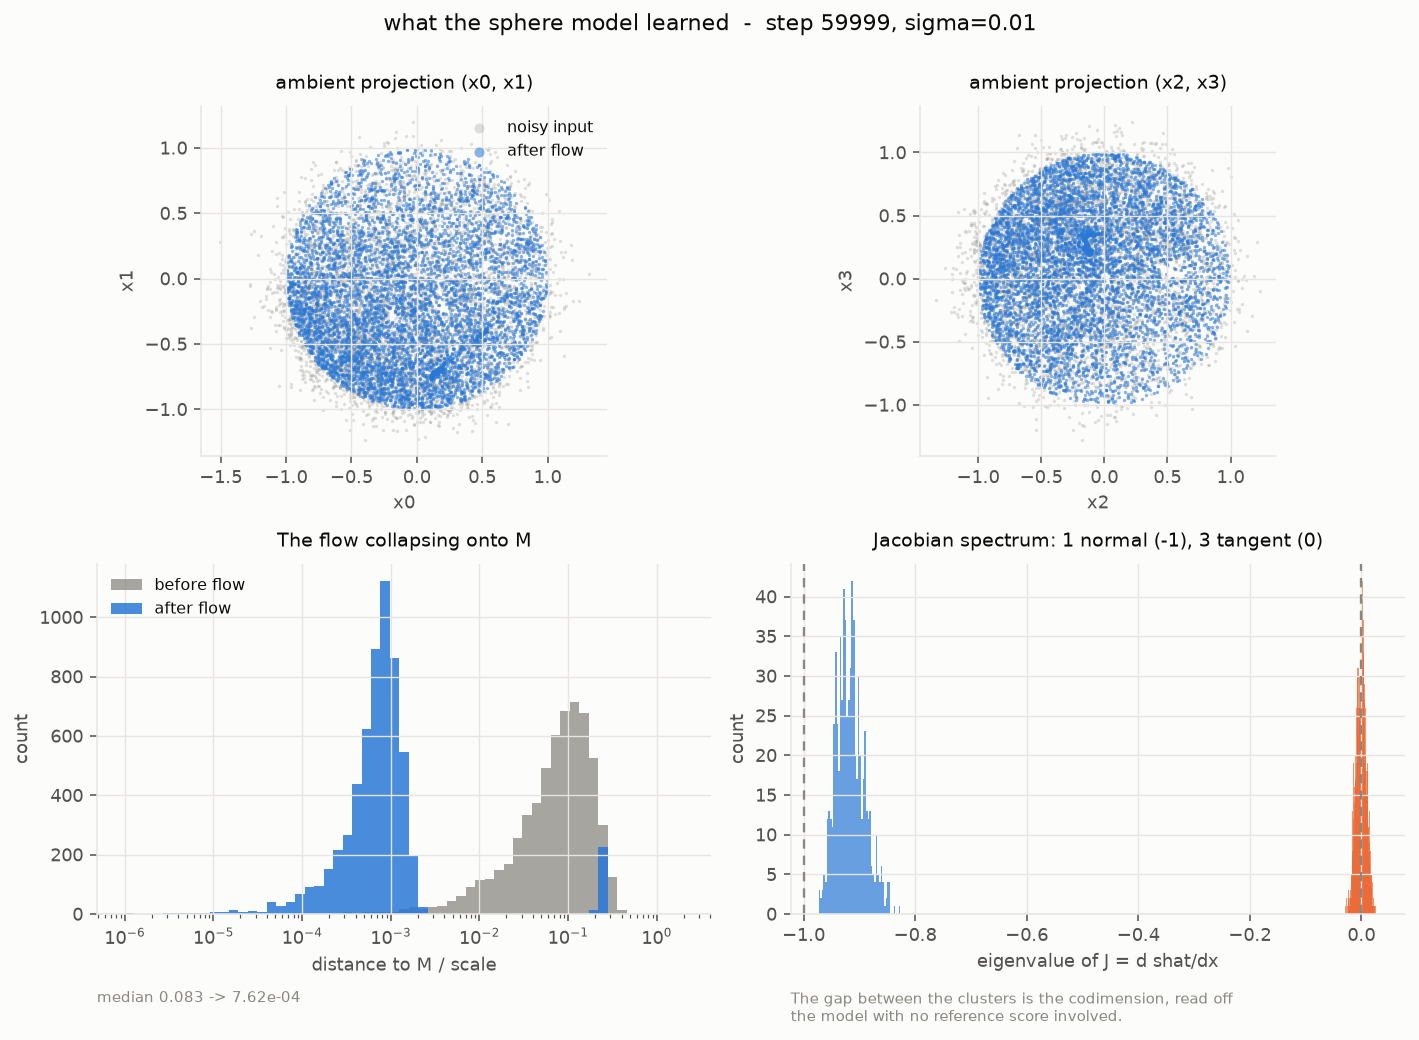
\includegraphics[width=\textwidth]{figures/sphere_learned.png}
\caption{The learned manifold. Distance to $M$ before/after the deterministic
flow (median $7.9{\times}10^{-4}$), and the spectrum of
$\partial\shat/\partial x \approx -P_\perp$, whose eigenvalue gap ($-0.92$
vs.\ $-0.0005$) identifies codimension~1 at every probe.}
\label{fig:learned}
\end{figure}

\begin{figure}[t]
\centering
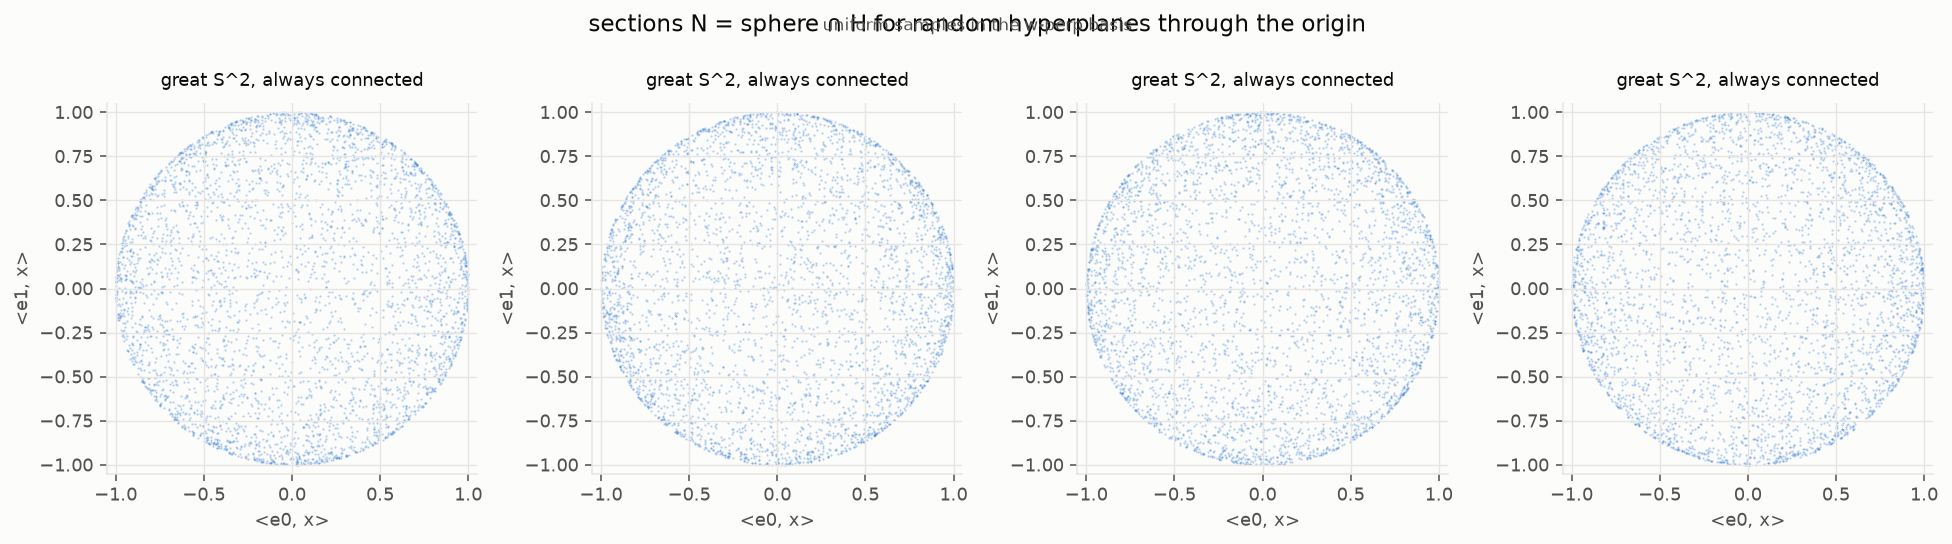
\includegraphics[width=0.8\textwidth]{figures/sphere_sections.png}
\caption{Sections $N = S^3 \cap H$ for random hyperplanes, as uniform samples in
an orthonormal basis of $w^\perp$: always a connected great $S^2$. Klein-bottle
sections instead have 2--4 components; disconnection freezes between-component
mass and is the failure mode there.}
\label{fig:sections}
\end{figure}

\begin{figure}[t]
\centering
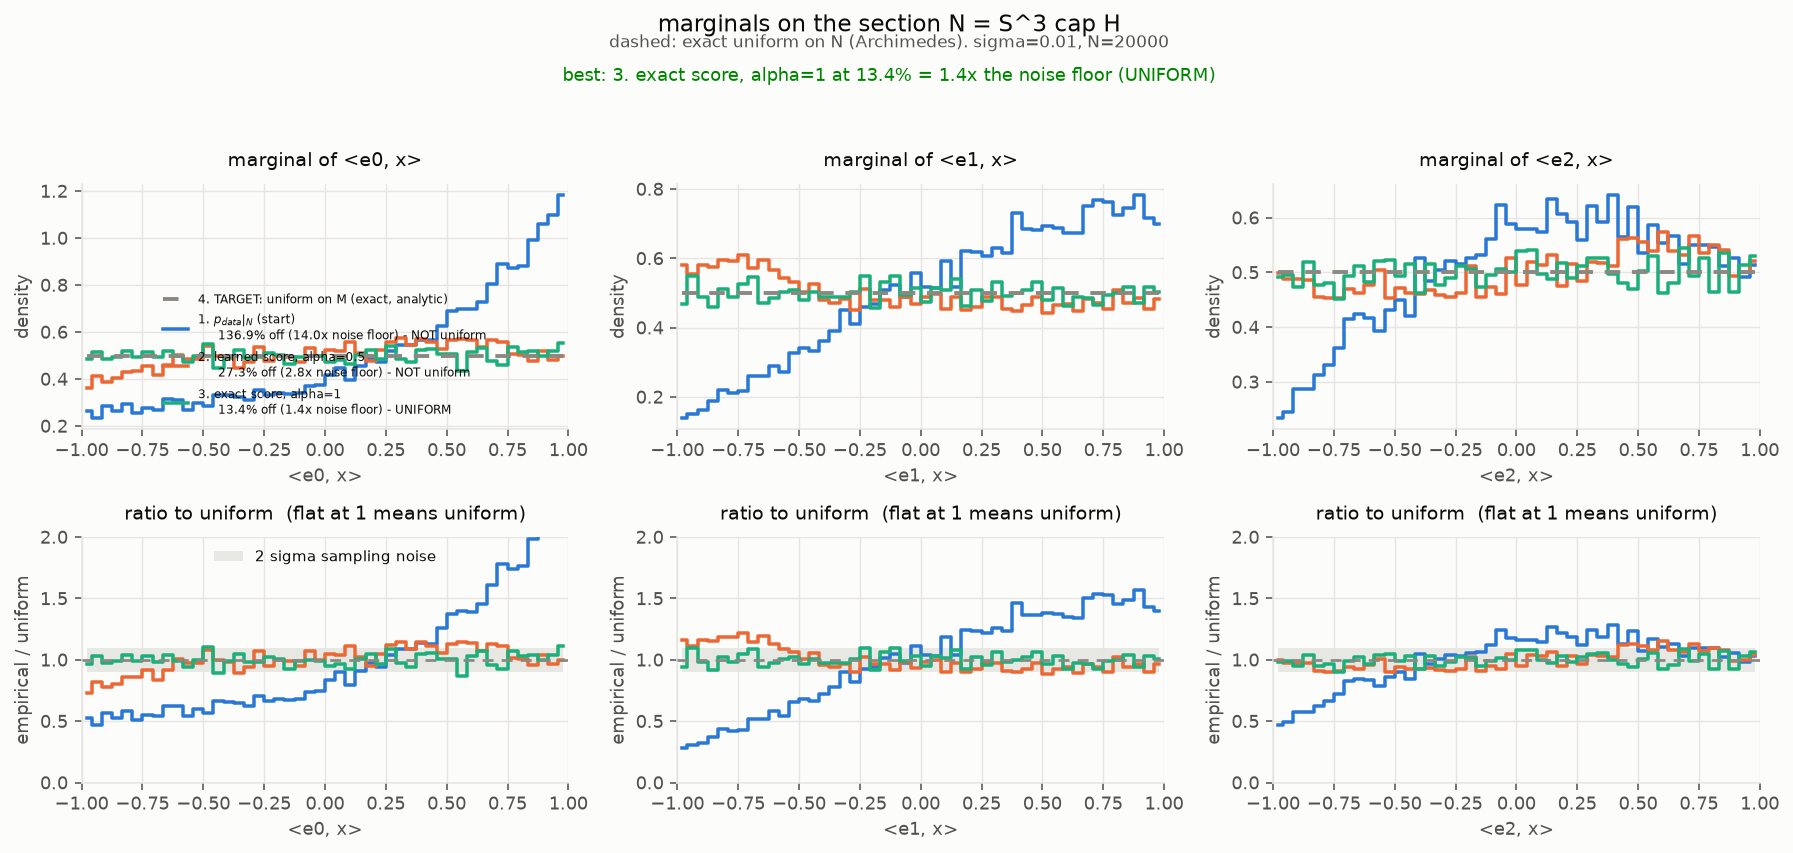
\includegraphics[width=\textwidth]{figures/sphere_uniformity.png}
\caption{Marginal histograms of $\langle e_k, x\rangle$ on the section (top) and
their ratio to the uniform density (bottom; flat at 1 means uniform), against the
analytic target (dashed).}
\label{fig:unif}
\end{figure}

\begin{figure}[t]
\centering
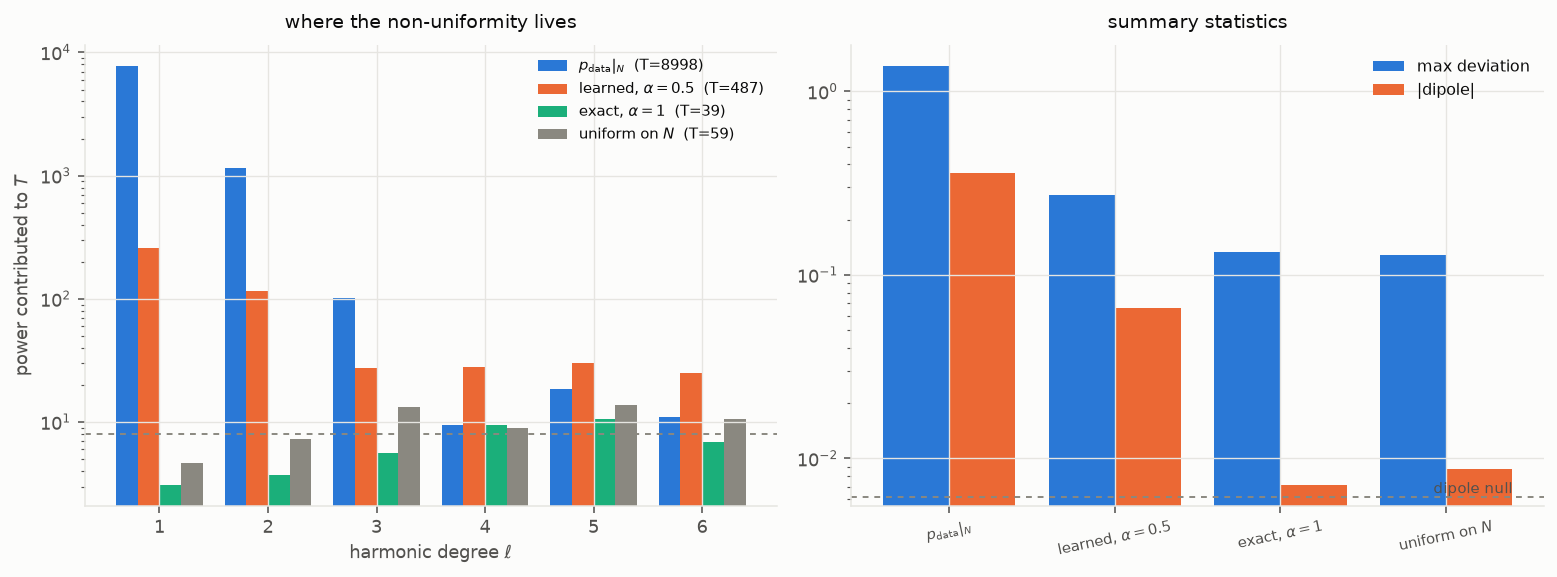
\includegraphics[width=\textwidth]{figures/sphere_spectrum.png}
\caption{Left: harmonic power per degree $\ell$. $\pdata|_N$ is a dipole plus
quadrupole; the exact-score sampler is at the noise level at every degree; the
learned-score residual is dominated by a single $\ell=1$ mode. Right: summary
statistics on a log scale against the dipole null.}
\label{fig:spec}
\end{figure}

\begin{figure}[t]
\centering
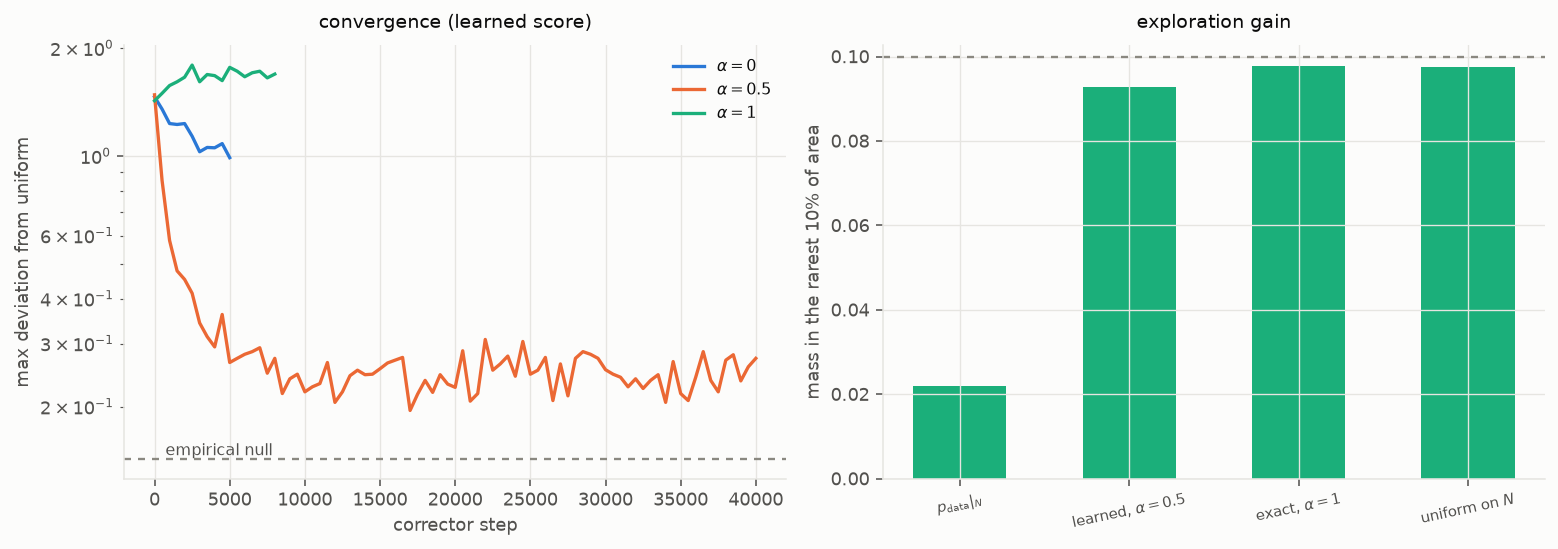
\includegraphics[width=\textwidth]{figures/sphere_convergence.png}
\caption{Left: convergence of the learned-score corrector; the $\alpha = 0$
control holds the restriction, as Theorem 5.1 requires ($\alpha=0$ is excluded).
Right: mass in the rarest 10\% of the section's area.}
\label{fig:conv}
\end{figure}

\section{Limitations}

Exact guidance exploits linearity of the constraint; class-conditional targets
need a learned $p(c\mid x_t,\sigma)$, and a softmax head measured here produces a
guidance term two orders of magnitude too small. All uniformity claims are at
$N_s = 20000$, so ``uniform'' means uniform to within what this sample size
resolves. The reported rates are magnitudes at typical noised points, not the
stiffness exponents of \eqref{eq:expansion}. $S^3$ is maximally symmetric
($\|P_{T}w\| \equiv 1$, sections always connected); on the Klein bottle sections
have 2--4 components, between-component mass is frozen at initialisation, and no
tempering exponent repairs it --- a limitation of local dynamics on disconnected
supports, not of the rate separation.

\end{document}
